\documentclass[aspectratio=169]{beamer}
\usepackage{lmodern}
\usetheme{Madrid}
%\usecolortheme{giantoak}
\newcommand*\oldmacro{}
\let\oldmacro\insertshorttitle
\renewcommand*\insertshorttitle{\oldmacro\hfill\insertframenumber\,/\,\inserttotalframenumber}
\usepackage[framemethod=tikz]{mdframed}

\usepackage{beamerthemesplit}
\usepackage{textpos}
\usepackage{pgf}
%\logo{\pgfputat{\pgfxy(0,-.4)}{\pgfbox[right,base]{\includegraphics[height=1.0cm]{logo.jpg}}}}
%\newcommand{\nologo}{\setbeamertemplate{logo}{}}
\usepackage{booktabs}
\usepackage{graphicx}
\theoremstyle{principle}
\newtheorem*{principle}{Design Principle}


\titlegraphic{\includegraphics[width=1.0\paperwidth]{cool-wind-800px.jpg}}

\title{Amendments}
%\author[Jeremy Kedziora]{Wind Data Science Team\\
%\small{Uptake}}
\date{}

\begin{document}

%{
%%\nologo
%\begin{frame}
%    \maketitle
%\end{frame}
%}
%pages 1-7, 8-9, 14-15.


{
  \usebackgroundtemplate{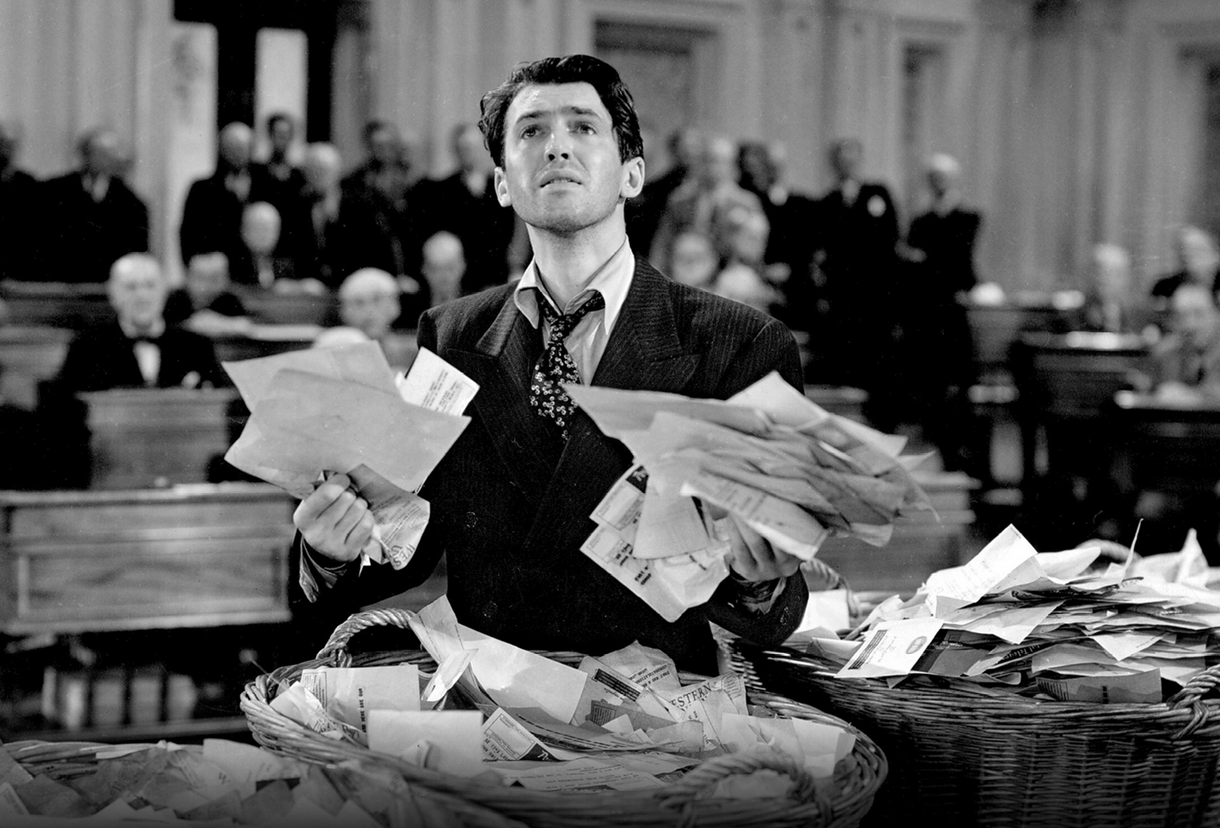
\includegraphics[width=1.0\paperwidth]{mr_smith.png}}
  \begin{frame}[plain]
  
\begin{mdframed}[tikzsetting={draw=black,fill=white,fill opacity=0.7,
               line width=0pt},backgroundcolor=none,leftmargin=20,
               rightmargin=20,innertopmargin=4pt]
\Huge Rethinking Representation
\end{mdframed}

  \end{frame}
}

%@@@@@@@@@@@@@@@@@@@@@@@@@@@@@@@@@@@@@@@@@@@@@@@@@
%\begin{frame}
%
%\begin{center}
%
\includegraphics[scale=0.4]{lake_michigan.jpg}
%\end{center}
%
%
%\end{frame}

%@@@@@@@@@@@@@@@@@@@@@@@@@@@@@@@@@@@@@@@@@@@@@@@@@
\begin{frame}

\begin{center}
\Huge \textbf{Are YOU well-represented?}%What is the role of representation?  Is the US a democracy?
\end{center}

\end{frame}

%@@@@@@@@@@@@@@@@@@@@@@@@@@@@@@@@@@@@@@@@@@@@@@@@@
\begin{frame}
\frametitle{Birkland$+$ Model of Policy, goals, problems}
\begin{itemize}
\item Policy Domain: what substantive problems are under consideration?  This specifies:
\begin{itemize}
\item The actors involved, official actors who can make decisions $+$ \textbf{stakeholders}; 
\item \textbf{Distribution of benefits/costs} $\Rightarrow$ actor organization, e.g. iron triangle, policy community;
\item The systemic agenda; 
\end{itemize}
\bigskip
\item \color{black}Input-output Model;
\begin{itemize}
\item Actors: \textbf{legislature, executive, bureaucrats, justices and the available levers};
\item Inputs: \textbf{agenda setting (application of power/social construction, focusing events, indicator change driven esp by unofficial actors)} \textbf{sets goals}, \textbf{determines the causal model}, which specifies the institutional agenda, and leads to the \textbf{policies} on the decision agenda;
\item Black box \textbf{decision making, timing (incrementalism, punctuated eq) driven by indicators/focusing events}, choice driven by e.g. median voter thm, Arrow's thm;
\begin{itemize}
\item Round 1: \textbf{works on decision agenda}, leads to outputs (e.g. statute laws, rules, court decisions);
\item Round 2: \textbf{Implementation}, leads to outcomes;
 \end{itemize}
\end{itemize}
\bigskip
\item Outcomes: \textbf{Feedback from failure and success}, learning leads to iteration and updates.
\end{itemize}
\end{frame}

%@@@@@@@@@@@@@@@@@@@@@@@@@@@@@@@@@@@@@@@@@@@@@@@@@
\begin{frame}
\frametitle{Purpose of the paper:}
\begin{itemize}
\item We (i.e. political scientists) have developed more sophisticated descriptions of the different ways that \textbf{representation} works;
\begin{itemize}
\item Promissory representation;
\item Anticipatory representation;
\item Gyroscopic representation;
\item Surrogate representation;
\end{itemize}
\bigskip
\bigskip
\item So for each of these what constitutes `good' representation?
\begin{itemize}
\item Expansion of knowledge above is positive -- normative has not kept up;
\item Goal of paper is to catch the normative up;
\end{itemize}
\bigskip
\bigskip
\item `Good' means some sort of effective accountability;
\begin{itemize}
\item Promissory has well-defined criteria but the rest do not meet it;
\item New criteria for the rest are \textbf{systemic rather than dyadic}...
\item ...and \textbf{plural rather than singular}.
\end{itemize}
\end{itemize}
\end{frame}

%@@@@@@@@@@@@@@@@@@@@@@@@@@@@@@@@@@@@@@@@@@@@@@@@@
\begin{frame}
\frametitle{Purpose of the paper:}
\begin{quote}
...analyzing each form separately makes it possible to identify the underlying power relation in each form, the role of deliberation in each, and the normative criteria appropriate to each. These normative criteria are goals toward which to strive... one might say that the closer a system of representation comes to meeting the normative criteria for democratic aggregation and deliberation, the more that system is normatively legitimate.
\end{quote}
\end{frame}

%@@@@@@@@@@@@@@@@@@@@@@@@@@@@@@@@@@@@@@@@@@@@@@@@@
\begin{frame}
\frametitle{Definitions}
\begin{itemize}
\item Power (\textbf{Dahl}): $A$ has power over $B$ to the extent that $A$ can get $B$ to do something $B$ would not otherwise do;
\bigskip
\bigskip
\item Power (\textbf{Nagel}): causal relation between the preferences of an actor regarding an outcome and the outcome itself;
\bigskip
\bigskip
\item \textbf{Retrospective Voting}: voters look back when deciding how to vote;
\bigskip
\bigskip
\item \textbf{Aggregative Democracy}: adding voters preferences up to make a decision;
\bigskip
\bigskip
\item \textbf{Deliberative Democracy}: the conversation.


\end{itemize}
\end{frame}



%@@@@@@@@@@@@@@@@@@@@@@@@@@@@@@@@@@@@@@@@@@@@@@@@@
\begin{frame}
\frametitle{Promissory Representation: power, deliberation, accountability}
\begin{itemize}
\item This is the baseline model that came along first;
\bigskip
\bigskip
\item Follows the principal--agent problem:
\begin{itemize}
\item Control advantage allows the agent to deviate from the principal's goals;
\item Information advantage allows the agent to deviate from the principal's goals;
\end{itemize}
\bigskip
\bigskip
\item Two flavors:
\begin{itemize}
\item \textbf{Mandate}: representative promises to follow constituents instructions/desires;
\item \textbf{Trustee}: representative promises to further constituents long-run interests and interest of the nation as a whole.
\end{itemize}
\end{itemize}

\end{frame}

%@@@@@@@@@@@@@@@@@@@@@@@@@@@@@@@@@@@@@@@@@@@@@@@@@
\begin{frame}
\frametitle{Promissory Representation: power, deliberation, accountability}
\begin{itemize}
\item Power relationship between voters and representative is linear in time:
\begin{itemize}
\item Voter at time $1$ extracts a promise from representative (election);
\item Representative at time $2$ implements policy (governing period);
\item Voter at time $3$ rewards or sanctions representative (election);
\item Clearly involves retrospective voting;
\end{itemize}
\bigskip
\bigskip
\item Reflects Dahl and requires forward looking intentionality;
\begin{itemize}
\item Voters ($A$) want to get representative ($B$) to make policy they would not otherwise;
\item Accountability comes through electoral sanctions;
\item Comes closest to an ideal where will of citizens is translated into policy;
\end{itemize}
\bigskip
\bigskip
\item Normative standard: `good' representation equals kept promises.
\end{itemize}

\end{frame}

%@@@@@@@@@@@@@@@@@@@@@@@@@@@@@@@@@@@@@@@@@@@@@@@@@
\begin{frame}
\frametitle{Anticipatory Representation: power, deliberation, accountability}
\begin{itemize}
\item Representative tries to please future voters;
\bigskip
\item Power relationship is backwards or non-linear;
\begin{itemize}
\item Voter at time $1$ extracts a promise from representative (election);
\item Representative is aware of the fact that voters may opt for a retrospective frame during future elections...
\item ...has \textbf{beliefs} about future voter preferences...
\item ...and \textbf{attempts to ensure those voters are satisfied with policy} at time 2 (governing period);
\item Voter at time $3$ rewards or sanctions representative (election);
\end{itemize}
\bigskip
\item Reflects more generalized power of Nagel and is derived from a marketplace model (see Stone); 
\bigskip
\item Two cases to consider:
\begin{itemize}
\item Voter preferences are stable $\Rightarrow$ no important difference between anticipatory and promissory;
\item Voter preferences are unstable $\Rightarrow$ representative has incentives to search for time 3 voter characteristics.
\end{itemize}
\end{itemize}

\end{frame}

%@@@@@@@@@@@@@@@@@@@@@@@@@@@@@@@@@@@@@@@@@@@@@@@@@
\begin{frame}
\frametitle{Anticipatory Representation: power, deliberation, accountability}
\begin{itemize}
\item Empirical implications -- redirects attention from time 1 to time 3:
\begin{itemize}
\item Representative has incentives to attempt to change time 3 voters $\Rightarrow$ model become \textbf{more deliberative} -- communications cycles;
\item Representative has incentives to engage \textbf{interests rather than policy preferences};
\item \textbf{Voters can be educated} by representatives, parties, interest groups, media, etc;
\end{itemize}

\item Normative implications -- accountability mechanisms have to be forward looking:
\begin{itemize}
\item Representative is entrepreneurial, trying to attract votes of future customers $\Rightarrow$ \textbf{prudential relationship w/ future voters};
\item Communication between representative and voter depends on entire system $\Rightarrow$ \textbf{what should system do}?
\item Representative has incentives to try to change voter preferences $\Rightarrow$ is this \textbf{education or manipulation}?
\end{itemize}

\item Representative anticipatory actions should be judged by three criteria:
\begin{itemize}
\item Non-manipulation -- no misleading voters;
\item Illumination of interests -- as opposed to policy preferences;
\item Retrospectively approvable transformation -- use of power to change the situation would be approved of by voters.
\end{itemize}
\end{itemize}

\end{frame}

%@@@@@@@@@@@@@@@@@@@@@@@@@@@@@@@@@@@@@@@@@@@@@@@@@
\begin{frame}
\frametitle{Gyroscopic Representation}
\begin{itemize}
\item Representatives act in ways the voter approves of without external incentives;
\bigskip
\item Representative looks within: understanding of interests, interpretive schemes, conscience, principles;
\bigskip
\item Voters seek to elect a `good' type:
\begin{itemize}
\item A single issue representative;
\item Commitment to the common good;
\item Character;
\item Party ID;
\item Descriptive characteristics;
\end{itemize}
\bigskip
\item Voters affect political outcomes by \textbf{inducing systemic preferences rather than individual preferences} $\Rightarrow$ power is over the system;
\bigskip
\item Note: may account for as much as 75\% of all voter-representative relationships;
\begin{itemize}
\item Most important mechanism for President and Senate;
\item Most important mechanism for House is anticipatory.
\end{itemize}
\end{itemize}

\end{frame}

%@@@@@@@@@@@@@@@@@@@@@@@@@@@@@@@@@@@@@@@@@@@@@@@@@
\begin{frame}
\frametitle{Gyroscopic Representation}
\begin{itemize}
\item Power relationship between voter and representative is over once election is finished -- they do not relate as principals and agents;
\begin{itemize} 
\item Key to voter ability to affect outcomes is \textbf{predictability} -- ability to construct good estimates of how a representative will act;
\item Party ID can help with this;
\item Reputation, descriptive characteristics, and character;
\end{itemize}
\bigskip
\bigskip
\item \textbf{Voter expects discretion} from representative:
\begin{itemize}
\item Representative is expected to act as voter would wish;
\item Empowers creative deliberation, e.g. compromise, changes of mind, etc. are allowed;
\end{itemize}
\bigskip
\bigskip
\item Normative implications:
\begin{itemize}
\item Accountability is irrelevant;
\item Ongoing communication between voters and representative is irrelevant;
\item Deliberation at authorization (no intentional deception during election) is really important $\Rightarrow$ predictability, illumination of interests;
\item Ease of maintenance and removal.
\end{itemize}
\end{itemize}

\end{frame}

%@@@@@@@@@@@@@@@@@@@@@@@@@@@@@@@@@@@@@@@@@@@@@@@@@
\begin{frame}
\frametitle{Surrogate Representation}
\begin{itemize}
\item Representation by representative with no electoral relationship -- e.g. a representative from another district;
\bigskip
\bigskip
\item Why would a representative give any attention to non-constituents?
\begin{itemize}
\item Campaign contributions;
\item In-kind services, volunteer time, information, expertise;
\item A felt sense of responsibility, e.g. gender, race/ethnicity, class, occupational similarity, etc.
\end{itemize}
\bigskip
\bigskip
\item The only power relationship between voters and representatives is the threat to withhold;
\begin{itemize}
\item Creates possibility for significant political inequality given campaign finance laws.
\end{itemize}
\end{itemize}

\end{frame}

%@@@@@@@@@@@@@@@@@@@@@@@@@@@@@@@@@@@@@@@@@@@@@@@@@
\begin{frame}
\frametitle{Surrogate Representation}
\begin{itemize}
\item Dyadic voter--representative accountability is irrelevant;
\bigskip
\bigskip
\item Normative implications -- the legislature as a whole should should represent the perspectives of the public in proportion;
\begin{itemize}
\item \textbf{Adversary representation}: aggregative aims of democracy mean that most conflictual interests get representation;
\item \textbf{Deliberative representation}: deliberative aims of democracy mean perspectives most important to a decision be represented during decision making -- but not necessarily proportionally;
\end{itemize}
\bigskip
\bigskip
\item Note: these are systemic criteria.
\end{itemize}

\end{frame}

%@@@@@@@@@@@@@@@@@@@@@@@@@@@@@@@@@@@@@@@@@@@@@@@@@
\begin{frame}
\frametitle{Conclusion}
\begin{itemize}
\item Good deliberation is required for each representation form to work effectively;
\bigskip
\bigskip
\item Each form of representation also has effects on deliberation:
\begin{itemize}
\item Anticipatory: communication between public and representatives probably has follow-on effects of legislature deliberation;
\item Gyroscopic: selection of individuals who deliberate well;
\item Surrogate: inclusion of varied perspectives;
\end{itemize}
\bigskip
\bigskip
\item No form is normatively `best' and so no normative criteria for `good' representation should eclipse the others.
\end{itemize}

\end{frame}

%@@@@@@@@@@@@@@@@@@@@@@@@@@@@@@@@@@@@@@@@@@@@@@@@@
\begin{frame}

\begin{center}
\Huge\textbf{Why should we care?}\\
\bigskip
\bigskip
\large Whenever you are advising an elected official these sorts of feedback effects will structure their receptivity to your recommendations.  In this sense, gyroscopic representatives may be simultaneously the easiest and most difficult to manage -- all you need to do is convince them.\\
\end{center}

\end{frame}

\end{document}






